 \documentclass[a4paper,fleqn,usenatbib]{mnras}
  
%font
\usepackage{newtxtext,newtxmath}
% Depending on your LaTeX fonts installation, you might get better results with one of these:
%\usepackage{mathptmx}
%\usepackage{txfonts}

% Use vector fonts, so it zooms properly in on-screen viewing software
% Don't change these lines unless you know what you are doing
\usepackage[T1]{fontenc}
\usepackage{ae,aecompl}

% Only include extra packages if you really need them. Common packages are:
\usepackage{graphicx}	% Including figure files
\usepackage{amsmath}	% Advanced maths commands
\usepackage{amssymb}	% Extra maths symbols

%\usepackage{caption} %doesn't work!!!!!
\usepackage{threeparttable}

\newcommand{\revisit}{\textcolor{red}}

\graphicspath{{figures/}}
 
%%%%%%%%%%%%%%%%%%%%%%%%%%%%%%%%%%%%%%%%%%%%%%%%%%

%%%%% AUTHORS - PLACE YOUR OWN COMMANDS HERE %%%%%

% Please keep new commands to a minimum, and use \newcommand not \def to avoid
% overwriting existing commands. Example:
%\newcommand{\pcm}{\,cm$^{-2}$}	% per cm-squared

%%%%%%%%%%%%%%%%%%%%%%%%%%%%%%%%%%%%%%%%%%%%%%%%%%

%%%%%%%%%%%%%%%%%%% TITLE PAGE %%%%%%%%%%%%%%%%%%%

% Title of the paper, and the short title which is used in the headers.
% Keep the title short and informative.
\title[SZ effect in SHELA cluster candidates]{Draft: The Atacama Cosmology Telescope: SZ-based masses of IR-selected cluster candidates from the SHELA survey}

% The list of authors, and the short list which is used in the headers.
% If you need two or more lines of authors, add an extra line using \newauthor
\author[B. Fuzia et al.]{
Brittany Fuzia,$^{1}$\thanks{E-mail: bjf13d@my.fsu.edu}
Lalitwadee Kawinwanichakij,$^{2}$
Eli Rykoff,$^{3}$
Nicola Mehrtens,$^{2}$
\newauthor ACT and SHELA collaborators, 
including
Kevin Huffenberger,$^1$ 
Casey Papovich$^{2}$, 
\newauthor Simone Aiola, Nicholas Battaglia, Mark Devlin, Megan Gralla, Matt Hilton, Jack Hughes,  
\newauthor Felipe Maldonado, Lyman Page, Bruce Partridge, Crist\'obal Sif\'on, Edward Wollack
\\
% List of institutions
$^{1}$Dept of Physics, Florida State University, Tallahassee, FL 32301, USA\\
$^{2}$Dept of Physics and Astronomy, Texas A\&M University, College Station, TX 77843, USA\\
$^{3}$ SLAC National Accelerator Laboratory, Menlo Park, CA 94025, USA\\
}

% These dates will be filled out by the publisher
\date{Accepted XXX. Received YYY; in original form ZZZ}

% Enter the current year, for the copyright statements etc.
\pubyear{2018}

% Don't change these lines
\begin{document}
\label{firstpage}
\pagerange{\pageref{firstpage}--\pageref{lastpage}}
\maketitle

% Abstract of the paper
\begin{abstract}
We examine the thermal Sunyaev-Zel\text{'}dovich (SZ) signals for a sample of galaxy cluster candidates from the Spitzer-HETDEX Exploratory Large Area (SHELA) Survey. 
The clusters are found in combined optical and infrared SHELA data using the redMaPPer algorithm. 
We separate the clusters into three richness bins: $10 \leq \lambda < 20$, $20 \leq \lambda < 30$, and $\lambda \geq 30$.
%, with richness being a measure of the number of galaxies in a cluster. 
From the lowest to highest richness bins, the average redshifts are 0.80, 0.73, and 0.70. 
The IR selection allows us to identify clusters at higher redshifts than typical for optical data alone, and objects less massive than those typical with SZ surveys. 
In the stacking analysis of Atacama Cosmology Telescope (ACT) data, the richest bin shows a clear temperature decrement at 148 GHz, which we attribute to the SZ effect.  All bins show an increment at 220 GHz, which we attribute to dust and radio emission. 
We correct for dust emission using stacked profiles from the Herschel Stripe 82 (HerS) survey. 
The profiles are extrapolated to the ACT frequencies based on a dust spectral energy distribution, which is fit to data from the HerS source catalog.
We correct for radio emission using a stacked profile created by binning source fluxes from NVSS.
We simultaneously fit for the dust, and radio, and SZ contributions, using a universal galaxy cluster pressure profile for the average SZ signal.
%For the highest richness bin, a mean mass of $M_{500} = (8.9^{+2.6}_{-2.6}) \times 10^{13}$ $M_{\odot}$ is obtained. 
Correcting for this dust and radio emission, we find that on average that the SZ mass is 1.8 times larger than when neglecting to correct it, indicating a partial fill-in of the SZ decrement from thermal dust and radio emission by the cluster member galaxies. 
We compare our SZ masses to two redMaPPer-based cluster richness scaling relations and find that the SZ mass is lower than predicted by the richness, even after correcting for dust and radio emission. 
We discuss possible explanations for this discrepancy, and note that the SHELA richnesses differ from previous richness measurements due to the inclusion of IR data in redMaPPer.


%We find a high stellar-to-total mass fraction in all richness bins. 
\end{abstract}

% Select between one and six entries from the list of approved keywords.
% Don't make up new ones.
\begin{keywords}

\end{keywords}

%%%%%%%%%%%%%%%%%%%%%%%%%%%%%%%%%%%%%%%%%%%%%%%%%%

%%%%%%%%%%%%%%%%% BODY OF PAPER %%%%%%%%%%%%%%%%%%


%%%%%%%%%%%%%%%%%%%%%%%%%%%%%%%
%INTRODUCTION
%%%%%%%%%%%%%%%%%%%%%%%%%%%%%%%
\section{Introduction}
Clusters of galaxies are the largest gravitationally bound structures in the universe. They make powerful cosmological probes because they sample the maxima of the primordial density field.  Various observable scaling laws make clusters useful tools to gain insight into large-scale structure, galaxy evolution, dark matter dynamics, and cosmological parameters \citep{2005RvMP...77..207V,2013SSRv..177..247G}. The thermal Sunyaev-Zel'dovich (SZ) spectral distortion of the Cosmic Microwave Background (CMB) allows for indirect measurements of one of the most important observables---total galaxy cluster mass---and can identify clusters to high redshift \citep{1972CoASP...4..173S, 2002ARA&A..40..643C}. 
The SZ effect occurs when CMB photons scatter from the hot electron gas in the intracluster medium. Fewer than $\sim$1 percent of photons interact and gain energy through inverse Compton scattering, altering the observed CMB spectrum and resulting in a characteristic spectral dependence for the SZ effect: a flux decrement for frequencies below 217 GHz and a flux increment for higher frequencies \citep{1999PhR...310...97B,2002ARA&A..40..643C}.
The magnitude of the effect is proportional to the Comptonization parameter (the integrated electron pressure), and the pressure is proportional to the depth of the gravitational potential well.  Therefore the amplitude of the SZ signal closely depends on the mass of the cluster.
Using the SZ effect for cosmology requires an understanding of this relationship between halo mass and the SZ observable, which is often expressed as the Comptonization parameter integrated over the cluster's solid angle. 
Since the SZ effect is a distortion of the CMB's spectrum, the signal does not decrease with distance the way that the cluster emission does, and so the SZ effect is an efficient way to find high-redshift clusters, limited only by the mass of the cluster and the sensitivity of the telescope.

At high mass, $M \gtrsim 10^{15}$ $M_\odot$, current SZ searches can already find halos efficiently at all redshifts, but at lower mass, $M \lesssim 10^{14}$ M$_{\odot}$, it becomes more difficult. 
These lower mass halos are interesting because their smaller potential wells have a harder time holding onto their gas, and are laboratories for star formation and AGN feedback \citep{2011ApJ...736...39H, 2013ApJ...767...38S, 2013A&A...555A..66L, 2015MNRAS.448.2085L}.  
Although studies of low mass halos using the SZ effect will become more common as CMB telescopes become more sensitive, for now we depend on stacking, or averaging, multiple clusters that have been detected by other means.  
Spatially coherent stacking enables allows the use of the SZ effect to extend to lower masses, as it averages out contributions from the CMB, atmosphere, and detector noise \citep{2013ApJ...767...38S, 2011A&A...536A..12P, 2011ApJ...736...39H}.

At low redshift, optical surveys can identify clusters efficiently with multiband overdensity finders: e.g., MaxBCG \citep{2007ApJ...660..221K}, redMaPPer \citep{2014ApJ...785..104R}, and CAMIRA \citep{2014MNRAS.444..147O}.
At higher redshift, the infrared becomes an efficient avenue of detection: e.g., MaDCoWS \citep{2014ApJS..213...25S,2018arXiv180906820G}, ISCS 
\citep{2008ApJ...684..905E}, IDCS \citep{2012ApJ...753..164S}, RCS \citep{2000AJ....120.2148G}, and several Spitzer catalogs \citep{2008ApJ...676..206P, 2010ApJ...716.1503P}.

The SZ signal of low-richness, optically-selected clusters is smaller than expected from mass--richness relationships, which are usually calibrated with high-richness clusters \citep{2011A&A...536A..12P,2012PhRvD..85b3005D,2013ApJ...767...38S,2016arXiv160508770S}. 
Several possible explanations for this discrepancy are: radio or infrared point source contamination of the SZ signal, line-of-sight projections contaminating richness measurements, cluster miscentering, variable gas mass fractions in optically selected clusters, or more fundamentally, a lower amplitude for the mass-richness relation.
Solving this discrepancy is vital so that scaling relations for clusters, and therefore cluster physics, are understood over a wide mass range, allowing clusters to be used to their full cosmological potential.

In this work, we look for the SZ signal in data from the Atacama Cosmology Telescope (ACT), using cluster candidates selected by the redMaPPer algorithm from catalogs of multiwavelength imaging, including Spitzer data from the SHELA survey.
The resulting sample is higher in redshift and lower in mass than many other samples. 
Using Herschel and NRAO VLA Sky Survey (NVSS) data, we correct the stacked SZ decrement for contamination from dust and radio emission, while simultaneously fitting for a halo mass based on the stacked SZ signal and characterizing the uncertainty with a Markov Chain Monte Carlo.
We also compare the sample's SZ masses to optical mass-richness relationships.

We adopt the flat $\Lambda$CDM cosmology from the Planck 2013 data release \citep{2014A&A...571A..16P} with $H_{0}$ = 67.9 km s$^{-1}$ Mpc$^{-1}$, $\Omega_{\rm m}$ = 0.307, $\Omega_{\rm \Lambda}$ = 0.693. 
The  mass $M_{500}$ is measured out to $R_{500}$, which is the radius enclosing 500 times the critical density at a given redshift.


This paper is organized as follows: In Section \ref{sec:data} we introduce the cluster sample, the ACT and ACTPol data, the Herschel data, and the NVSS data used in this analysis. 
In Section \ref{sec:methods} we describe the methods we used to analyze the data. 
These include the filtering and stacking procedures, calculation of the covariance matrices, and a discussion of the noise and signals that contribute to the stacked profiles. 
We describe our resulting multifrequency stacked profiles 
%in Section \ref{sec:multifreqprof}, 
and discuss our methods for removing dust and radio contamination. 
We describe our fitting procedure, including the SZ and pressure profile we use to translate our SZ signal into a cluster mass. 
In Section \ref{sec:results}, we present the results of our analysis and discuss how our SZ masses scale with richness. 
In Section \ref{sec:conclusions}, we conclude with a summary of the analysis and results.


%%%%%%%%%%%%%%%%%%%%%%%%%%%%%%% 
%DATA 
%%%%%%%%%%%%%%%%%%%%%%%%%%%%%%% 
\section{Data} \label{sec:data}

\subsection{Cluster Sample}

\begin{table}
  \centering
  \caption{Properties of the SHELA cluster candidate richness bins}
%  \begin{threeparttable}
  \begin{tabular}{|*{4}{c|}}
    \hline
    & $10 \leq \lambda < 20$ & $20 \leq \lambda < 30$ & $\lambda \geq 30$ \\ \hline
    
    N$_{\rm clusters}$ & 840 & 172 & 70 \\ \hline
     
    $z$ range & 0.50--1.60 & 0.50--1.35 & 0.52--1.18  \\ \hline
    
    average $z$ & 0.80 & 0.73 & 0.70 \\ \hline
    
    $\lambda$ range & 10--20 & 20--30 & 30--76 \\ \hline %\hline
    
    average $\lambda$ & 14 & 24 & 39 \\ \hline
    
    \end{tabular}
  %\begin{tablenotes}
%	\item fff
%  \end{tablenotes}
%  \end{threeparttable}
\label{table:sampleinfo}
\end{table}


The sample contains IR- and optically-selected redMaPPer cluster candidates from the Spitzer-HETDEX Exploratory Large Area survey  \citep{2016ApJS..224...28P}. 
SHELA is a 24 deg$^2$ IRAC survey in a low IR background region of Stripe 82 \citep{2000AJ....120.1579Y}, centered at a right ascension of 1$^{\rm h}$22$^{\rm m}$00$^{\rm s}$ on the celestial equator, and extending $\pm$6.5$^{\circ}$ in right ascension and $\pm$1.25$^{\circ}$ in declination. 
The SHELA survey region also includes DECam $ugriz$ imaging. Multiwavelength coverage in the same field includes SDSS and HETDEX in the optical, NEWFIRM in K-band, Herschel in the sub-mm, and ACT in the microwave. 

The IR and optical imaging are passed through the redMaPPer algorithm \citep{2014ApJ...785..104R}, resulting in a catalog of 1082 groups and clusters with a richness $\lambda \geq 10.$ 
For more information on the SHELA catalog, see \cite{2019ApJS..240....5W}.
Richness is a measure of how many galaxies belong to a cluster. 
In redMaPPer, it is defined as the sum of the membership probabilities for the galaxies within a cluster. 
We use clusters with richnesses $\lambda \geq 10$, and break these into three richness bins: $10 \leq \lambda < 20$, $20 \leq \lambda < 30$, and $\lambda \geq 30$. 
{There are 840, 172, and 70 clusters in the lowest to highest richness bins, respectively.} 
Two rich clusters from the SHELA sample have already been detected in the ACT SZ cluster sample in this area of the sky \citep{2013JCAP...07..008H}.  
None of the remaining objects are detected individually in SZ by ACT, so their individual masses must be roughly $\leq$ $10^{14}$ M$_\odot$, ACT's approximate mass limit.
In this redshift range, $\sim$0.7--0.8, the 90\% completeness limit for $M_{500}$ in ACT is 4--5 $\cdot 10^{14}$ M$_{\odot}$ \citep{2018ApJS..235...20H}.   
Properties of each richness bin are summarized in Table \ref{table:sampleinfo}.


\subsection{ACT Millimeter-Wave Data}
We use ACT data to measure the SZ decrement and null signals. 
ACT is a six-meter millimeter wave telescope that resides at an altitude of 5200 meters on Cerro Toco in the Chilean Atacama Desert. 
It surveys the CMB with high resolution and sensitivity. 
The first generation of ACT observations dates from 2007-2010; there were three detector arrays operating at frequencies of 148, 220, and 277 GHz. 
These bands were chosen to study the SZ and capture the SZ decrement, null, and increment. 
ACT surveyed two regions on the sky, the ``southern'' and ``equatorial'' surveys. 
The southern survey covered 455 deg$^2$ and is centered on declination -53.5$^{\circ}$ \citep{2011ApJ...731..100M}. 
The equatorial region overlaps with 270 deg$^2$ of Stripe 82 and the entire SHELA survey, covering 504 deg$^2$ and spanning from 20$^{\rm h}$16$^{\rm m}$00$^{\rm s}$ to 3$^{\rm h}$52$^{\rm m}$24$^{\rm s}$ in right ascension and -2$^{\circ}$07$^{\prime}$ to 2$^{\circ}$18$^{\prime}$ in declination \citep{2013JCAP...07..008H}. 
The second generation of the experiment, ACTPol, was deployed in 2013.  It has receivers at 90 and 148 GHz, polarization capability,  and triple the sensitivity of ACT. 
ACTPol has made observations in four deep field patches and one wider field and continues to take data \citep{2014JCAP...10..007N,2018ApJS..235...20H}. 
The wider ``Deep 5/6'' region overlaps with SHELA, covers 548 deg$^2$, is centered on the celestial equator, and expands the area covered by ACT.\footnote{ACT and ACTPol maps are available for download from \url{https://lambda.gsfc.nasa.gov/product/act/}}
In this work, we measure the SZ decrement using coadded, point source subtracted, ACT temperature maps at 148 GHz from all observing seasons that overlap with the SHELA survey region: seasons 3--4 (2009 and 2010) of ACT and season 2 (2014) of ACTPol. 
The ACT maps have 0.495 arcmin pixels, while the ACTPol maps have 0.5 arcmin pixels. 
We use ACT maps that have been repixelized into the ACTPol pixelization to make coadded maps of all available data. %\citep{2011ApJS..194...41S}??. 
From seasons 3--4 of ACT, we use data at 220 GHz, a frequency near the SZ null, to constrain contamination from thermal dust and radio emission. 
These maps are also repixelized into the ACTPol pixelization. 
At FWHM, the beam sizes are 1.4 arcmin at 148 GHz, and 1.0 arcmin at 220 GHz.

\subsection{Herschel Submillimeter Data}
To measure dust emission from cluster member galaxies, we use far-IR data from the Herschel Stripe 82 (HerS) survey, which consists of maps at 250, 350, and 500 $\mu$m (or 1200, 857, 600 GHz) observed with \textit{Herschel}/SPIRE \citep{2014ApJS..210...22V}. 
The survey covers 79 deg$^2$, spanning 13$^{\circ}$ to 37$^{\circ}$ in right ascension and -2$^{\circ}$ to +2$^{\circ}$ in declination. 
The SPIRE beams are 18.2, 25.2, and 36.3 arcsec at 1200, 857, 600 GHz, respectively. 
In addition to the maps, in this work we use the band-merged source catalog from the HerS team, which contains compact source flux densities and uncertainties in each band. 
The HerS team assumed sources are point-like and they identified them using the IDL software package STARFINDER \citep{2000A&AS..147..335D}. 
They produced the band-merged catalog using the De-blended SPIRE Photometry (DESPHOT) algorithm, which uses source positions from the 1200 GHz band as a prior for the other frequencies \citep{2010MNRAS.409...48R}.

\subsection{NVSS Radio Data}
To measure radio emission from cluster member galaxies, we use 1.4 GHz data from the NRAO VLA Sky Survey (NVSS), which covers the sky North of declination -40$^{\circ}$ \citep{1998AJ....115.1693C}.
We use flux densities and uncertainties from the source catalog, which contains around 10$^6$ sources brighter than approximately 2.5 mJy.


%%%%%%%%%%%%%%%%%%%%%%%%%%%%%%%
%METHODS
%%%%%%%%%%%%%%%%%%%%%%%%%%%%%%%
\section{Methods} \label{sec:methods}

Our overall strategy in this analysis is to build up a model for the stacked emission in the ACT bands at the location of the clusters, allowing for SZ, dust, and radio components.  
We estimate the data's covariance due to CMB and noise fluctuations, and then use a Markov Chain Monte Carlo to estimate the parameters of our emission model.

\begin{figure*}
\centering
  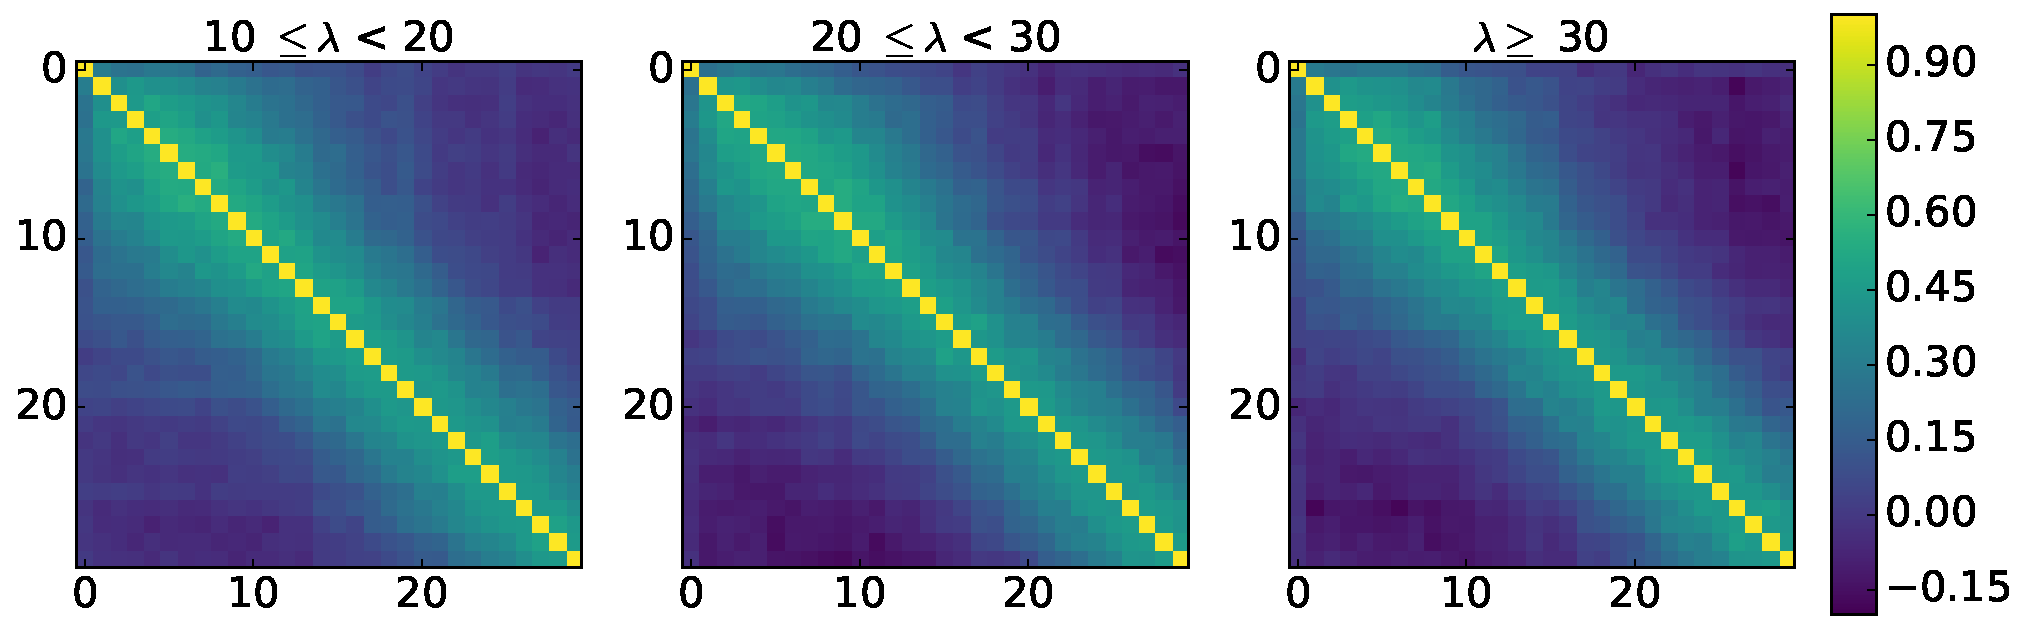
\includegraphics[width=1.75\columnwidth]{correlation_1600_coadd_act_actpol_148_tophat_zbin01_all.pdf}
  \caption{Correlation matrices for the stacked pressure profiles at 148 GHz for the three richness bins, $10 \geq \lambda < 20$ (left), $20 \leq \lambda < 30$, and $\lambda \geq 30$ (right). They are obtained by stacking on 1600 ACT simulations which contain correlations introduced by CMB fluctuations, detector and atmospheric noise for the different observing seasons of ACT used in this analysis. The axes label the radial bin numbers.}
  \label{fig:covariance}
\end{figure*}

\subsection{SZ Profiles}
The SZ signal can be expressed as a change in CMB temperature by: 
\begin{equation}
\centering
  \frac{\Delta T}{T_{\rm CMB}} = y( \theta ) \, f( x ) ,
\end{equation}
where $x = {h \nu}/{k T_{\rm CMB}}$ and $f(x) = x ({e^{x} + 1})/{(e^{x}-1)} - 4$ contains the frequency dependence of the SZ effect in the non-relativistic limit. The Compton parameter $y$ is proportional to pressure integrated along the line of sight \citep{1972CoASP...4..173S,1970CoASP...2...66S}:
\begin{equation}
  y(\theta) = \frac{\sigma_{T}}{m_{e} c^{2}} \int dl\  P(\theta, l) . \end{equation}
To translate our stacked temperature profile into a mass measurement, we use the universal pressure profile (UPP) of \cite{2010A&A...517A..92A} [A10], which is calibrated using low-redshift X-ray clusters from REXCESS \citep{2007A&A...469..363B}. 
A10 fit a generalized Navarro-Frenk-White profile which allows for a normalization that varies with mass and redshift and a mass-dependent deviation from self-similarity in the shape of the profile. 
In this model, the pressure at any radius $r$ (or $x' \equiv r/R_{500}$) is:

\begin{equation}
P(r) = P_{500} \bigg[ \frac{M_{\rm SZ,500}}{3x10^{14} h^{-1}_{70} M_{\odot}} \bigg]^{\alpha_{p} + \alpha^{\prime}_{p}(x')} \textbf{p}(x') \ h^{2}_{70} \ keV \ cm^{-3}
\end{equation}
where $P_{500}$ is the normalization of the pressure profile at the radius where the density is 500 times the critical density at a given redshift,
\begin{equation}
P_{500} = 1.65 \times 10^{-3} E(z)^{8/3} \bigg[\frac{M_{500}}{3 \times 10^{14} h_{70}^{-1} M_{\odot}}\bigg]^{2/3} h_{70}^2 keV cm^{-3},
\end{equation}
$E(z)$ is the evolution of the Hubble parameter, \textbf{p}$(x')$ is the dimensionless universal pressure profile,
\begin{equation}
\textbf{p}(x') = \frac{P_{0}}{(c_{500} x')^{\gamma} [1 + (c_{500} x')^{\alpha}]^{(\beta-\gamma)/\alpha}}
\end{equation}
and $\alpha^{\prime}_{p}(x')$ describes the deviation from self-similiarity,
\begin{equation}
\alpha^{\prime}_{p}(x') = 0.10 - (\alpha_{p} + 0.10) \frac{(x'/0.5)^{3}}{1. + (x'/0.5)^{3}}
\end{equation}
with $\alpha_p$ = 0.12.
Using local clusters with XMM-Newton data, \cite{2013A&A...550A.131P} update the best-fit parameters for the UPP to [$P_{0},c_{500},\gamma,\alpha,\beta$] = [6.51,1.81,0.31,1.33,4.13], which we adopt in this paper.


\subsection{Map Filtering and Stacking}
Before stacking, we filter the maps using a conservative high-pass filter designed to remove large scale CMB fluctuations while minimally altering the small scale cluster signal. 
To avoid bias, we design a filter independent of any assumed cluster shape.
Our filter is a Fourier-space high-pass filter that we define in terms of its low-pass complement.  
The low-pass complement in real space is an apodized top-hat. 
It is unity inside $3'$ radius and tapers to zero outside of $5'$ with a cosine transition. 
Thus our high-pass filter removes the large scale features in the map, and barely touches small harmonic scales. 
Our filter is not matched to any specific cluster profile, and leaves much of the small-scale detector white noise in the data.  
When compared, all maps, simulations, and model cluster profiles are subjected to this same filter. 

Our results are robust to changes in this filter.  As a test, we modified the filter to introduce beam smoothing.  The filter is the same high-pass filter used for the analysis, but convolved with the beam at 148 GHz to reduce pixel-scale white noise. 
This resulted in smoother, shallower profiles, but the mass measurements were similar to those reported in this analysis, with higher uncertainty as there was more bin to bin correlation.

%\subsection{Stacking Procedure}
Most of the cluster candidates were not individually detected in SZ by ACT. 
To increase the signal-to-noise we stack, or average, observations of the clusters together into 30 annular bins, centered on the redMaPPer cluster positions, out to a radial separation of nine arcminutes. 
CMB and white noise fluctuations have zero mean, therefore stacking observations partially averages out these noise fluctuations. 
The center of each pixel determines where the measurement is binned.

We can write our stacked profiles as a sum of the beam-convolved signals ($(b \ast P)(\theta)$) and noise ($n$):
\begin{equation}
\begin{split}
      P^{148} & = b^{148} \ast ( P^{\rm SZ} + P^{\rm dust,148} + P^{\rm radio,148} + n^{\rm CMB} ) \\ & + n^{\rm det,148} + p_0^{148}
\end{split}
\label{eq:prof148}
\end{equation}

\begin{equation}
  \label{eq:prof220}
 \begin{split}
  P^{220} & = b^{220} \ast ( P^{\rm dust,220} + P^{\rm radio,220} + n^{\rm CMB} ) \\ & + n^{\rm det,220} + p_0^{220}
\end{split}
\end{equation}

The ACT beams that we use ($b^{148}, b^{220}$) include the smoothing effects of the pixel window and the telescope pointing jitter.
A model dust SED provides the scaling which allows us to extrapolate the HerS stacked profiles to 148 and 220 GHz.
There is little SZ signal at 220 GHz, so we can use this profile to estimate the contributions from dust and radio emission in the ACT bands. 
The models we use to estimate $P^{\rm dust}$ and $P^{\rm radio}$ are discussed in Sections \ref{sec:dustprof} and \ref{sec:radioprof}.

\subsection{Covariance Matrices}

In the ACT frequencies, 148 and 220 GHz, the error in each annular bin of the stacked profile reflects the covariance introduced by CMB fluctuations, detector noise, and atmosphere. 
The covariance matrix is calculated by carrying out the same filtering and stacking procedure on 1600 simulations that model coadded ACT and ACTPol maps. 
To do this, we repixelize the ACT maps into the new ACTPol pixelization, and make coadded maps of all of the different seasons and arrays. 
We use the power spectra of the coadded maps to generate CMB plus noise simulations that account for cross-correlations between 148 and 220 GHz.  
The simulations are then filtered the same way as the data. 
The covariance is largest in the small angle bins where there are few measurements to average down the noise. 
The correlation matrix is calculated by dividing out the diagonal of the covariance, and is shown for each richness bin at 148 GHz in Figure \ref{fig:covariance}, showing that there is mild correlation between the annular bins.  

Errors on the dust SED, dust profiles, and radio profiles also figure into our final uncertainties.  
The HerS catalog includes 1$\sigma$ uncertainties for the flux density of each source, which we use by averaging in quadrature for the SED fitting process. 
The error bars on the stacked Herschel profiles come from stacking on the survey's noise maps. 
The covariance of the stacked NVSS profile come from binning the variance of each source flux and smoothing with the appropriate ACT beam and filter to account for the appropriate bin-to-bin correlation.

\subsection{Multifrequency Profiles} \label{sec:multifreqprof}

\begin{figure*}
  \centering
  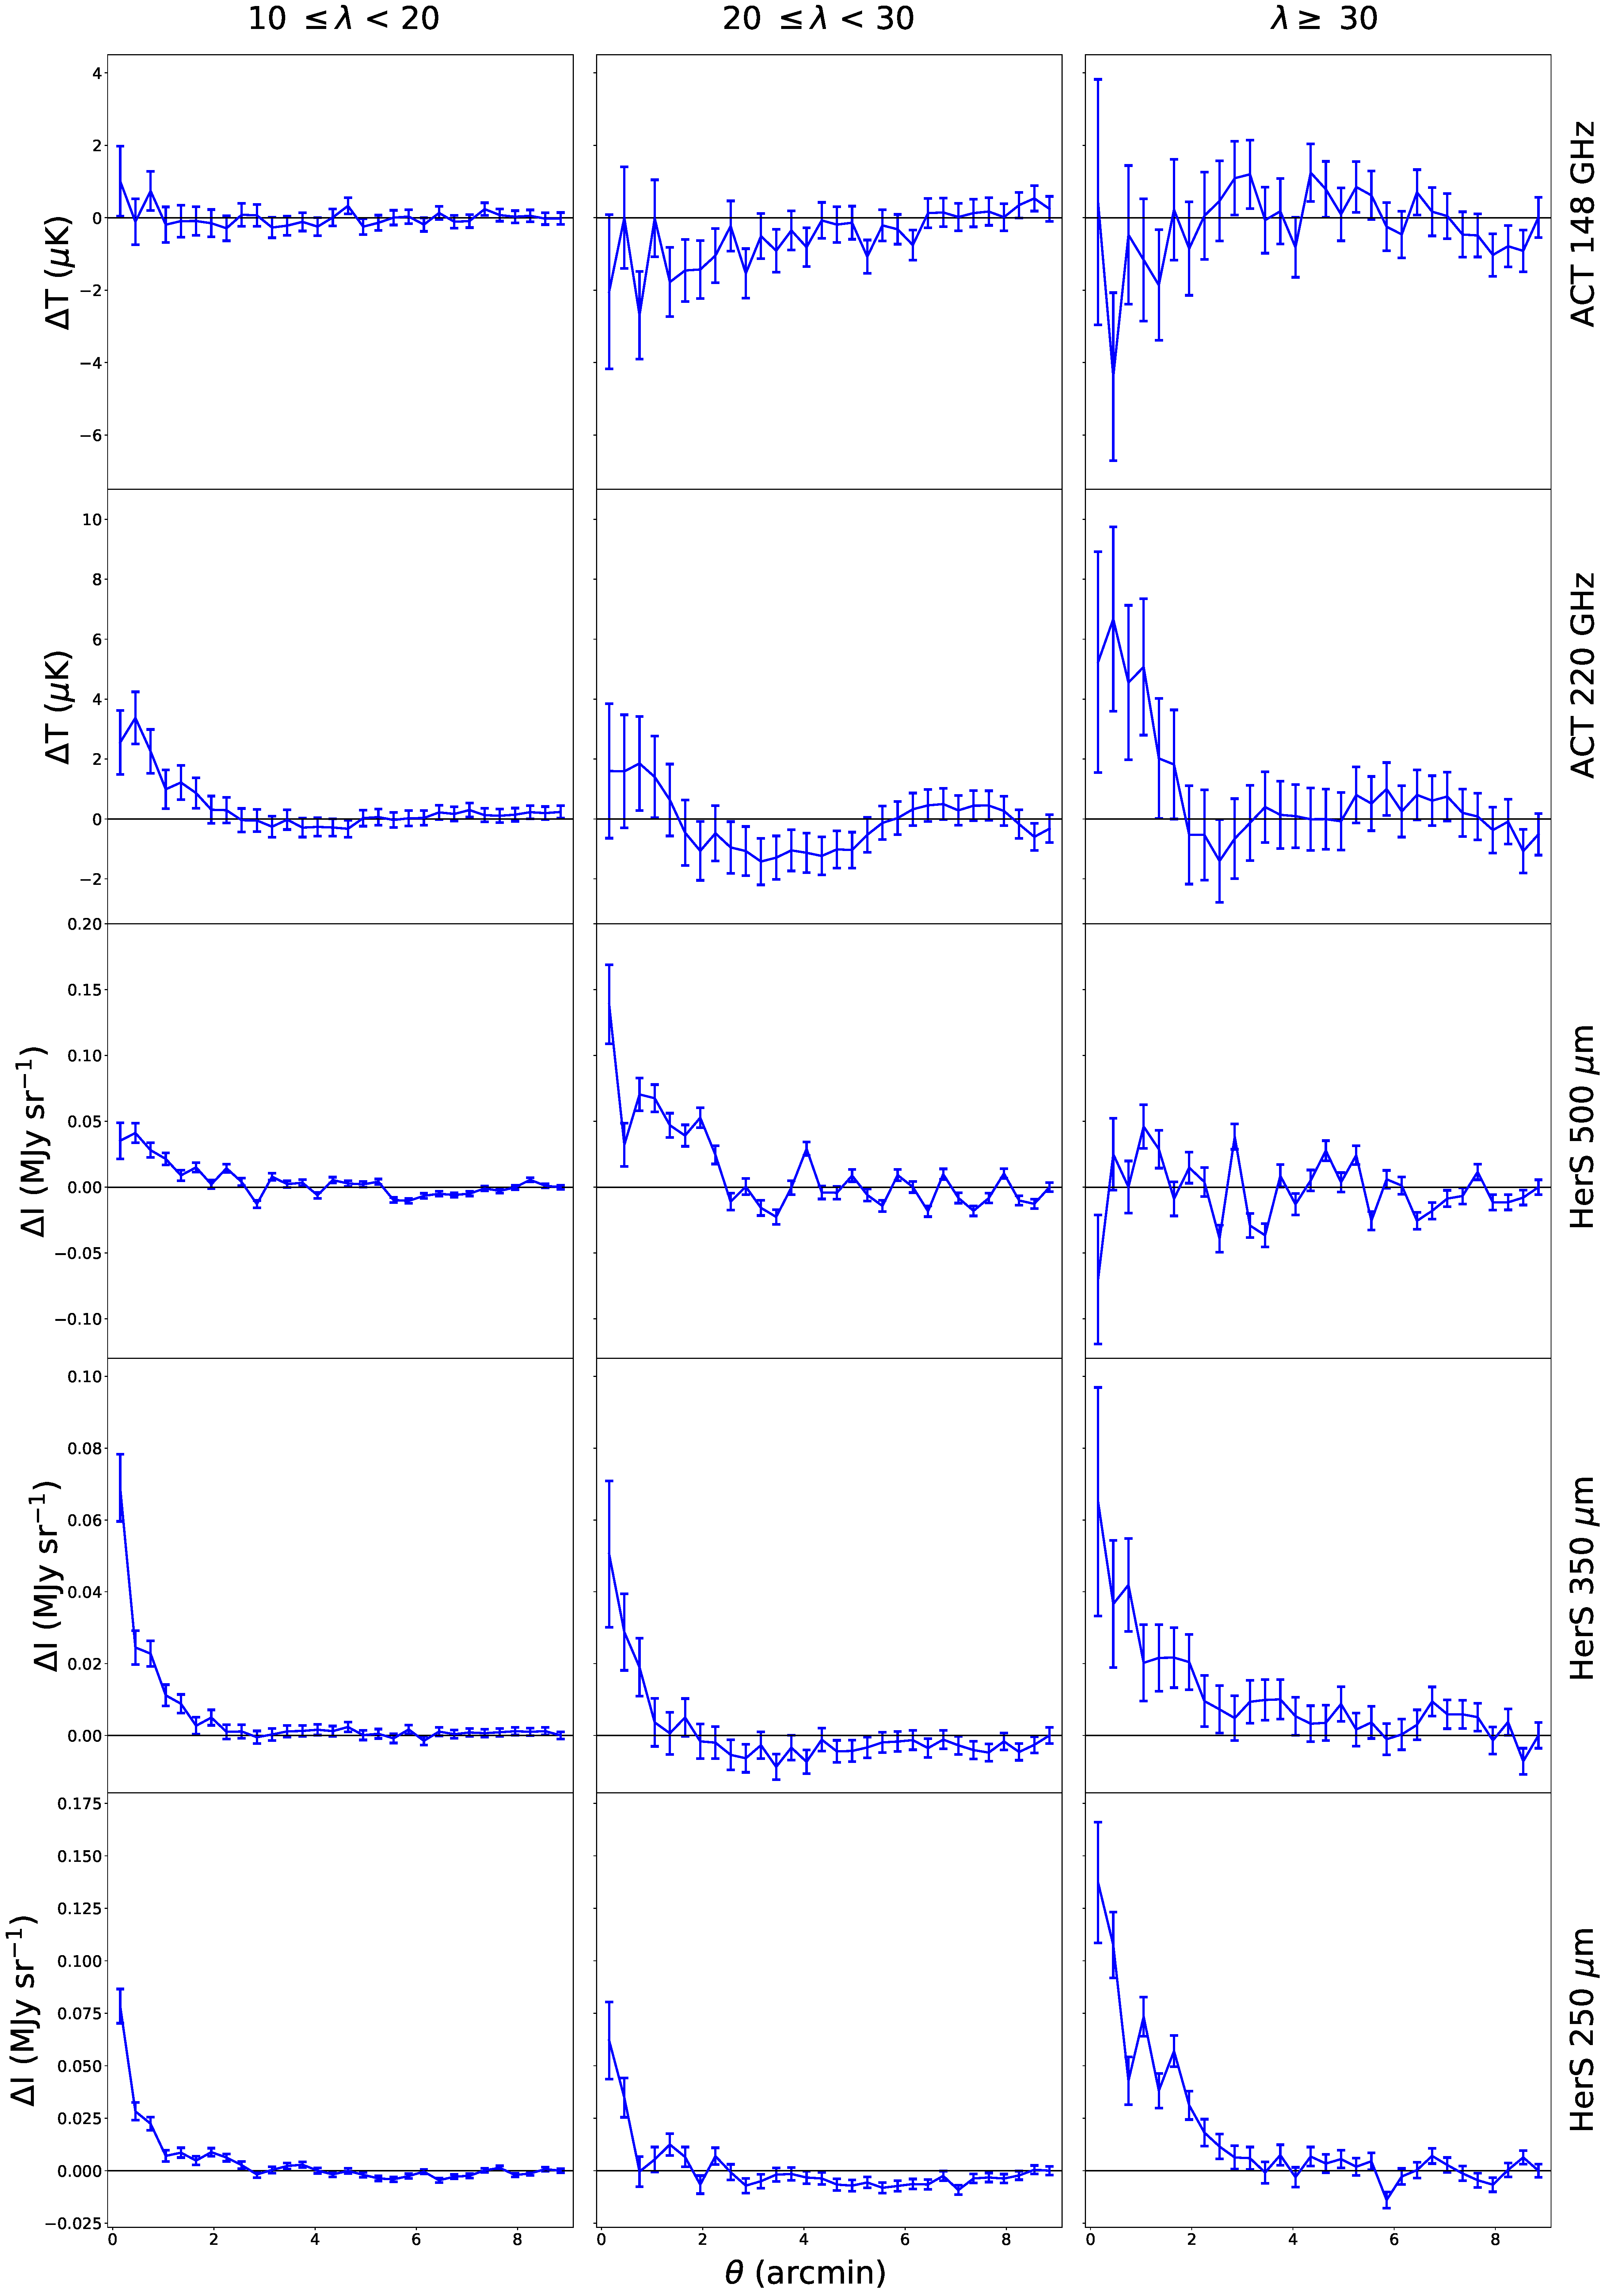
\includegraphics[height=0.9 \textheight]{5panel_rawprofs_all_stacks_all_rbin.pdf}

\caption{Stacked profiles for all 6 bands used in this analysis: NVSS 1.4 GHz, ACT 148 GHz, 220 GHz and HerS 500, 350, 250 $\mu m$ - for the three richness bins. 
The main contributions to the profile at 148 GHz are the SZ signal, plus some signal from dust and radio emission. 
ACT 220 GHz is near the SZ null, and contains emission which contaminates the signal at 148 GHz. 
The Herschel bands (500, 350, 250 $\rm \mu m$) trace thermal dust emission in the clusters. 
The NVSS stacks (filtered with the ACT 148 GHz beam and hi-pass filter) trace radio emission.  
The error bars are the diagonal of the covariances described in the text.
All profiles are filtered with the high-pass filter.
We plot our stacked profiles out to a radius of 5' to highlight the cluster centered emission.}  
  \label{fig:rawstacks}
\end{figure*}

\begin{figure}
  \centering
  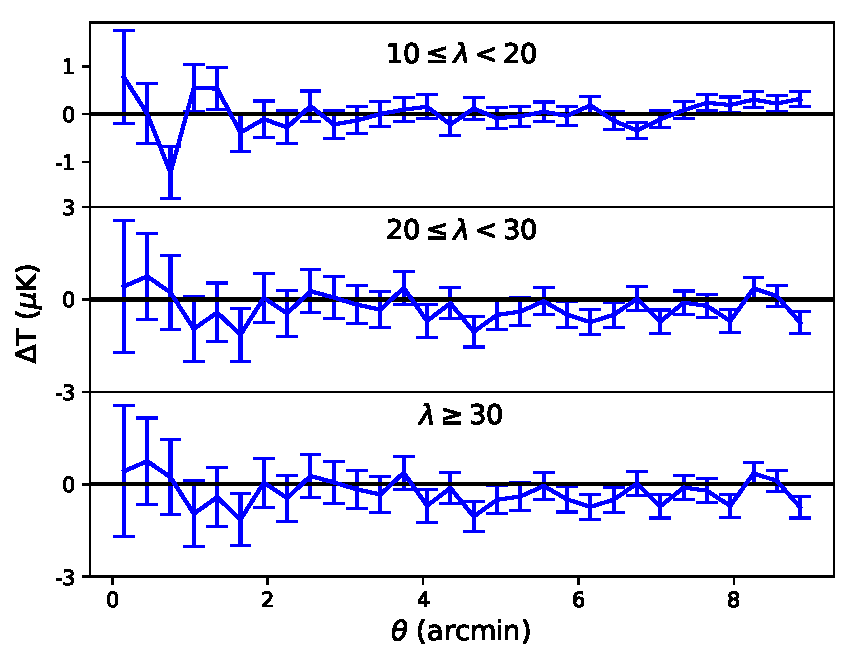
\includegraphics[width=0.45\textwidth]{rand_stacks_tophat.pdf}

\caption{Stacking null test at 148 GHz. We stack on random positions for the number of clusters in each richness bin to test that there is no signal in places unassociated with clusters.  {Although the bottom bin has an offset, it has the smallest number of objects and so is most subject to large scale fluctuations.  Assessed by the $\chi^2$, none of these samples have a significant signal.}}  
  \label{fig:randstacks}
\end{figure}




The stacked profiles for the different richness bins are shown in Figure \ref{fig:rawstacks}. 
The profiles show the cluster-centered emission for NVSS sources at 1.4 GHz, ACT at 148 and 220 GHz, and the three HerS bands (600--1200 GHz). 
%Compared to the other profiles, the radio profile is less smooth due to the contributions of individual bright source and the small VLA beam, and has small error bars that result from binning the variances of the sources from the NVSS catalog.  
When the radio profile is extrapolated to the ACT bands, it is convolved with the appropriate ACT beam and becomes much smoother.
Here we plot the radio profile and error bars smoothed with the 148 GHz beam.
The profiles at 148 GHz do not show an SZ decrement at very high significance, but it is subject to being filled in by the dust emission and radio emission, which are two mechanisms we want to constrain.
We expect the stacks at 220 GHz to contain little SZ signal, but they do show clear cluster-centered emission, as well as CMB and noise. 
We use this 220 GHz emission profile to constrain the dust and radio components. 
Also shown, and used to fit for dust, are profiles from stacking on the HerS maps at 500, 350, and 250 $\mu$m. 
We have fit for, and removed, an offset in the profiles at radii larger than 5'.
The error bars on the stacked profiles result from stacking on the noise maps provided with the HerS data. 
The ACT 220 GHz, NVSS, and Herschel stacks demonstrate that there is a signal from dust and radio emission within a few arcminute radius of the cluster centers.

To test the robustness of the noise model, and that our signals are not merely a feature caused by the stacking procedure, we stack on random positions in the ACT map, and find no signal on average. 
Figure \ref{fig:randstacks} shows the results from stacking on random positions in the 148 GHz map, with each null stack accounting for the number of clusters in the different richness bins.   %\revisit{in quadrature} -- ask about this
We use the full covariance to compute $\chi^2$.  The probability to exceed $\chi^2$ for the null hypothesis is 0.47, 0.45, and 0.35 respectively for the lowest to highest richness bin random null stacks.  
%The null stack for the lowest richness bin is the most stringent test of the noise model because of the large number of objects.  
%The somewhat low probability for the lowest richness comes from the positive signal at $\theta>7$ arcmin.  
%This may indicate that our noise model is lacking some feature at large scales, but we believe it is sufficiently accurate on the scales of the cluster, which is important for fitting the mass.


\subsection{Dusty Source Contamination}
\label{sec:dustprof}
Emission from dusty sources and radio sources contaminates the SZ signal in clusters \citep{2005A&A...439..901A}. As seen in Figure \ref{fig:rawstacks}, when stacking at 220 GHz (the SZ null) and higher frequencies there is an excess signal, which we partially attribute to dust emission from cluster member galaxies. 
This positive emission will also be present at 148 GHz, where it fills in the SZ decrement, causing the sample to appear to have less than its true mass. 
To correct for this, we fit for a dust component at 148 and 220 GHz.  

The dust profiles at 148 and 220 GHz take their shape from the HerS stacked profiles.  We have been extrapolated the three profiles to the ACT frequencies (using a dust SED that we fit to HerS sources), and then averaged them
\begin{equation}
    P^{\rm dust,\nu_{\rm ACT}} = \frac{1}{3} \big ( f^{250-\nu_{\rm ACT}} \cdot P^{250} + f^{350-\nu_{\rm ACT}} \cdot P^{350} + f^{500-\nu_{\rm ACT}} \cdot P^{500} \big )
\end{equation}
where $\nu_{\rm ACT}$ is either 148 or 220 GHz, and $f^{\nu_{\rm HerS}-\nu_{\rm ACT}}$ is the ratio of the flux density between the different HerS and ACT bands, which is determined by the dust SED.

For the dust SED, we fit a graybody SED using the source catalog from the HerS survey \citep{2014ApJS..210...22V}:
\begin{equation}
  \label{eq:dustSED}
  \centering
  S(\nu) = A_{\rm dust}  \bigg(\frac{\nu(1+z)}{\nu_0}\bigg)^{\beta_{\rm dust}} \frac{\big(\nu(1+z)\big)^{3} }{{\exp({h \nu (1+z) / k T_{\rm dust}}) - 1}}
\end{equation}
for an overall amplitude, $A_{\rm dust}$, and dust temperature, $T_{\rm dust}$, using the total contribution of all the sources within a fixed angular distance from the clusters. 
The Herschel source fluxes are used to infer $S(\nu)$, which is used to scale the Herschel stacks down to the ACT frequencies. 
We fix the emissivity spectral index $\beta_{\rm dust}$ to 1.5, $\nu_0$ to 100 GHz, and the redshift to the average redshift for each of the richness bins. 
\cite{2014A&A...561A..86M} find that setting $\beta_{\rm dust}$ to 1.5 is a good estimate when fitting spectra without enough information to constrain it, and note that it may cause $T_{\rm dust}$ to be slightly overestimated. 
Furthermore, when fitting for a stacked SZ plus greybody spectrum for Planck galaxy clusters, \cite{2018MNRAS.476.3360E} found that the choice of $\beta_{\rm dust}$ had little influence on the measured SZ signal, and use $\beta_{\rm dust}$ = 1.5 to obtain their main results. 
We ran our pipeline on the data from the highest richness bin using $\beta_{\rm dust}$ = 1.4 and 1.6 to see how $\beta_{\rm dust}$ affects our results. We found that varying $\beta_{\rm dust}$ did not significantly affect the mass measurements; the differences were less than 0.1$\sigma$. 
We report results with SED fitting to HerS sources with an 11' aperture in Table \ref{table:mcmcfitparam}, but the results are not sensitive to the precise aperture.



\subsection{Radio Source Contamination}
\label{sec:radioprof}
Radio sources have been found to reside preferentially in clusters of galaxies and are often associated with emission from the cluster member galaxies \citep{2002ApJ...580...36H,2007ApJS..170...71L,2007AJ....134..897C,2009ApJ...694..992L, 2011ApJ...734..103G}. 
Similarly to the process of measuring dust emission, we look for radio sources within 9' of the cluster centers and model their emission at 148 and 220 GHz. 
We use sources from the NVSS survey at 1.4 GHz \citep{1998AJ....115.1693C}. 
Our model for radio emission is:
\begin{equation}
  \label{eq:radioSED}
  \centering
  P^{\rm radio, \nu_{\rm ACT}} = A^{220}_{\rm radio} \cdot P^{1.4}_{\rm radio} \cdot \left(\frac{\nu_{\rm ACT}}{220 \ \rm GHz}\right)^{\alpha_{\rm radio}}  
\end{equation}
Where $A^{220}_{\rm radio}$ is an amplitude at 220 GHz, $\alpha_{\rm radio}$ is the spectral index which determines the frequency scaling, and $P^{1.4}_{\rm radio}$ is the normalized stacked radio profile.
The 1.4 GHz radio profile $P^{1.4}_{\rm radio}$ comes from summing the flux density of sources from the NVSS catalog into the bins used for all the stacking in this paper, and dividing the resulting profile by the solid angle in each bin. 
The profile is then normalized to unit integral over solid angle so that $A^{220}_{\rm radio}$ has dimensions of flux density.
When being compared to the stacks at 148 and 220 GHz, the model radio profile is filtered with the same filter used in the analysis, and smoothed by the beam for the appropriate ACT frequency.
Our data cannot constrain the spectral index, $\alpha$, so we apply a prior to our MCMC fitting procedure, which is based off of ACT and Planck measurements.
When using ACT data and fitting AGN for synchrotron, SZ, and IR emission, \cite{2014MNRAS.445..460G} measured $\alpha_{\rm radio} = -0.55 \pm 0.03$.
For a sample of DSFG's and AGN, \cite{2014MNRAS.439.1556M} find a spectral index between 148 and 218 GHZ of $\alpha^{148-218}_{\rm radio} = -0.55 \pm 0.60$.
\cite{2011ApJ...731..100M} find $\alpha^{20-148}_{\rm radio} = -0.39 \pm 0.04$ and $\alpha^{5-148}_{\rm radio} = -0.20 \pm 0.03$.
There have been several Planck studies measuring the spectral index of radio sources.
For several classes of radio sources, $\alpha_{\rm radio}$ was measured to range between $\sim$ -0.37 and -0.78  \citep{2016A&A...596A.106P}, and when scaling from 30 GHz, the spectral indices for extragalactic sources were measured to be -0.39 and -0.37 when scaling to 143 and 217 GHz respectively \citep{2011A&A...536A..12P}.
Given this information, we have designed a prior on $\alpha_{\rm radio}$ that is a Gaussian distribution with a mean of -0.5 and a standard deviation of 0.2.
We tested how adjusting the width of the distribution affects our SZ mass measurements.
Adjusting the prior's standard deviation to 0.1, 0.4, and 0.6 resulted in masses that were within 0.05 $\sigma$ of our original mass measurement, and did not affect the uncertainty in the measurement.



\section{Results} \label{sec:results}

We use a Markov-Chain Monte Carlo method to fit the stacked profile at 148 GHz and infer an $M_{500}$. We then use richness information available from the IR and optical data to compare to other works.



%%%%%%%%%%%%%%%%%%%%%%%%%%%%%%%
%RESULTS
%%%%%%%%%%%%%%%%%%%%%%%%%%%%%%%

\subsection{Mass Fitting}

\begin{table*}
   
  \centering
  \caption{Best-fit parameters for fitting an SZ profile in two ways: correcting for dust and radio emission, and neglecting dust and radio contamination.}
  \begin{threeparttable}
  \begin{tabular}{|*{10}{c|}}
    \hline
    & & \multicolumn{2}{|c}{$10 \leq \lambda < 20$} & & \multicolumn{2}{|c|}{$20 \leq \lambda < 30$} & & \multicolumn{2}{|c|}{$\lambda \geq 30$}\\ \hline
    
    & & Corr. & No corr. & \ &  Corr. & No corr. & \ &  Corr. & No dust corr. \\ \hline
    
    $M_{500}$ (10$^{13}$ M$_{\odot})$ & & $1.1^{+0.5}_{-1.1}$ & $0.9^{+0.2}_{-0.4}$ & \ & $2.7^{+1.5}_{-1.4}$ & $1.7^{+0.6}_{-1.2}$ & \ & $8.6^{+1.6}_{-1.4}$ & $6.6^{+1.4}_{-1.5}$ \\ \hline
     
    $p_0^{148} \ (\rm Jy/Sr)$ & & $-38.5^{+40.2}_{-37.9}$ & $-7.9^{+35.4}_{-35.4}$ & \ & $-40.3^{+76.8}_{-73.6}$ & $-3.9^{+78.7}_{-78.7}$ & \ & $-124.9^{+128.4}_{-112.7}$ & $-82.6^{+161.3}_{-149.5}$ \\ \hline
    
    $p_0^{220} \ (\rm Jy/Sr)$ & & $-21.0^{+62.5}_{-67.4}$ & - & \ & $-278.1^{+132.0}_{-138.3}$ & - & \ & $-243.2^{+225.1}_{-211.3}$ & - \\ \hline
    
    $T_{\rm dust} \ (\rm K)$ & & $29.1^{+0.50}_{-0.50}$  & - & \ & $28.0^{+0.11}_{-0.10}$ & - & \ & $27.0^{+0.16}_{-0.15}$ & - \\ \hline 

    $A^{220}_{\rm dust} \ (\rm mJy)$ & & $1.18^{+0.01}_{-0.01}$ & - & \ & $2.07^{+0.03}_{-0.03}$ & - & \ & $1.94^{+0.04}_{-0.04}$ & - \\ \hline
    

    $A^{220}_{\rm radio} \ (\rm mJy)$ & & $0.33^{+0.15}_{-0.29}$ & - & \ & $0.11^{+0.02}_{-0.11}$ & - & \ & $0.63^{+0.26}_{-0.56}$ & - \\ \hline
    
  \end{tabular}
  \begin{tablenotes}
	\item Resulting fit parameters for the three richness bins. 
	The first column for each richness bin shows results from fitting for dust and radio scaling simultaneously with the SZ profile, fixed at the average redshift for each sample, assuming no  mass bias. 
	The second column lists the results if we neglect the dust and radio correction and fit an SZ profile directly to the original stacked profile. 
	%The masses for the two lower richness bins are not significant, and their upper limits are discussed in the text.
  \end{tablenotes}
  \end{threeparttable}
\label{table:mcmcfitparam}
\end{table*}


To take into account the corrections in the mass fitting, we simultaneously fit for SZ, dust, and radio contributions to the stacked profiles. 
We use a Gaussian likelihood and the affine-invariant Markov Chain Monte Carlo code \textit{emcee} \citep{2013PASP..125..306F}. 
The fit parameters are the average cluster mass $M_{500}$, an overall DC offset for the stacked profile at 148 GHz and 220 GHz, $p_0^{148}$ and $p_0^{220}$, an amplitude for the graybody SED $A_{\rm dust}$, a dust temperature $T_{\rm dust}$, an amplitude for the radio scaling at 220 GHz $A_{\rm radio}^{220}$, and a spectral index for the radio scaling $\alpha_{\rm radio}$. 
We fix the redshift dependence of the dust spectrum (Equation 10) and SZ signal (Equation 4, and calculations of $R_{500}$ and $\rho_c$) to the average redshift for each sample, $z = 0.80, 0.73,$ and 0.70, for the lowest to highest richness bins. 
We apply a flat prior for values within the following ranges: 0 $M_{\odot} <  M_{500} < 10^{15} \rm M_{\odot}$,$\ -10 \mu$K $< p_0^{148} < +10 \mu$K, $\ -10 \mu$K $< p_0^{220} < +10 \mu$K, 0 Jy/Hz$^3$ $< A_{\rm dust}$ < $10^{15}$ Jy/Hz$^3$,$\ 3 $K $< T_{\rm dust} < 500$K, $A_{\rm radio}^{220}$ > 0 mJy.
The prior for $\alpha_{\rm radio}$ is a Gaussian centered on -0.5, with a standard deviation of 0.2, as discussed in Section \ref{sec:radioprof}. 
The HerS flux densities are used to sample the graybody SEDs, which determines how to scale the HerS profiles to 148 and 220 GHz. 
The HerS profiles are deconvolved with their respective beams and reconvolved with the appropriate ACT beams.
The shape of the radio profile is used with the sampled values for $A_{\rm radio}^{220}$ and $\alpha_{\rm radio}$ to estimate the radio contribution at 148 and 220 GHz.
The radio profile is convolved with the appropriate ACT beams.
For each step in the sampler, the sampled mass is used to calculate the SZ signal $y(\theta)$, which is convolved with the ACT beam and translated into a temperature profile, $\Delta T(\theta)$.
The sum of the SZ, dust, and radio signals are compared to the stacked profile at 148 GHz. 
The sum of the dust and radio signals are compared to the stacked profile at 220 GHz.

The SZ signal does not scale linearly with mass, and choosing one mass value to compare with our stacked profiles may cause us to infer a value for $M_{500}$ that is not characteristic of the clusters in the sample.
To address this, we tested a second fitting method that uses a weighted average of SZ profiles to compare with our stacked profile.
We start with the richness distribution of the clusters in each bin, and use the mass-richness relation of \cite{2015MNRAS.454.2305S} to translate the richness distribution into a mass distribution. 
For each $M_{500}^{\rm MCMC}$ that is sampled in the MCMC, we shift the mass probability density distribution to have a mean which is $M_{500}^{\rm MCMC}$, and scale the probabilities accordingly. 
Then we perform a weighted average of the SZ signal with a range of masses, where the weights are the probabilities from the new mass probability density distribution.
The masses that we infer from this fitting method differ from the masses inferred in the main analysis by less than 0.1$\sigma$, but this correction may be more important with higher S/N data.




\begin{figure}
  \centering
  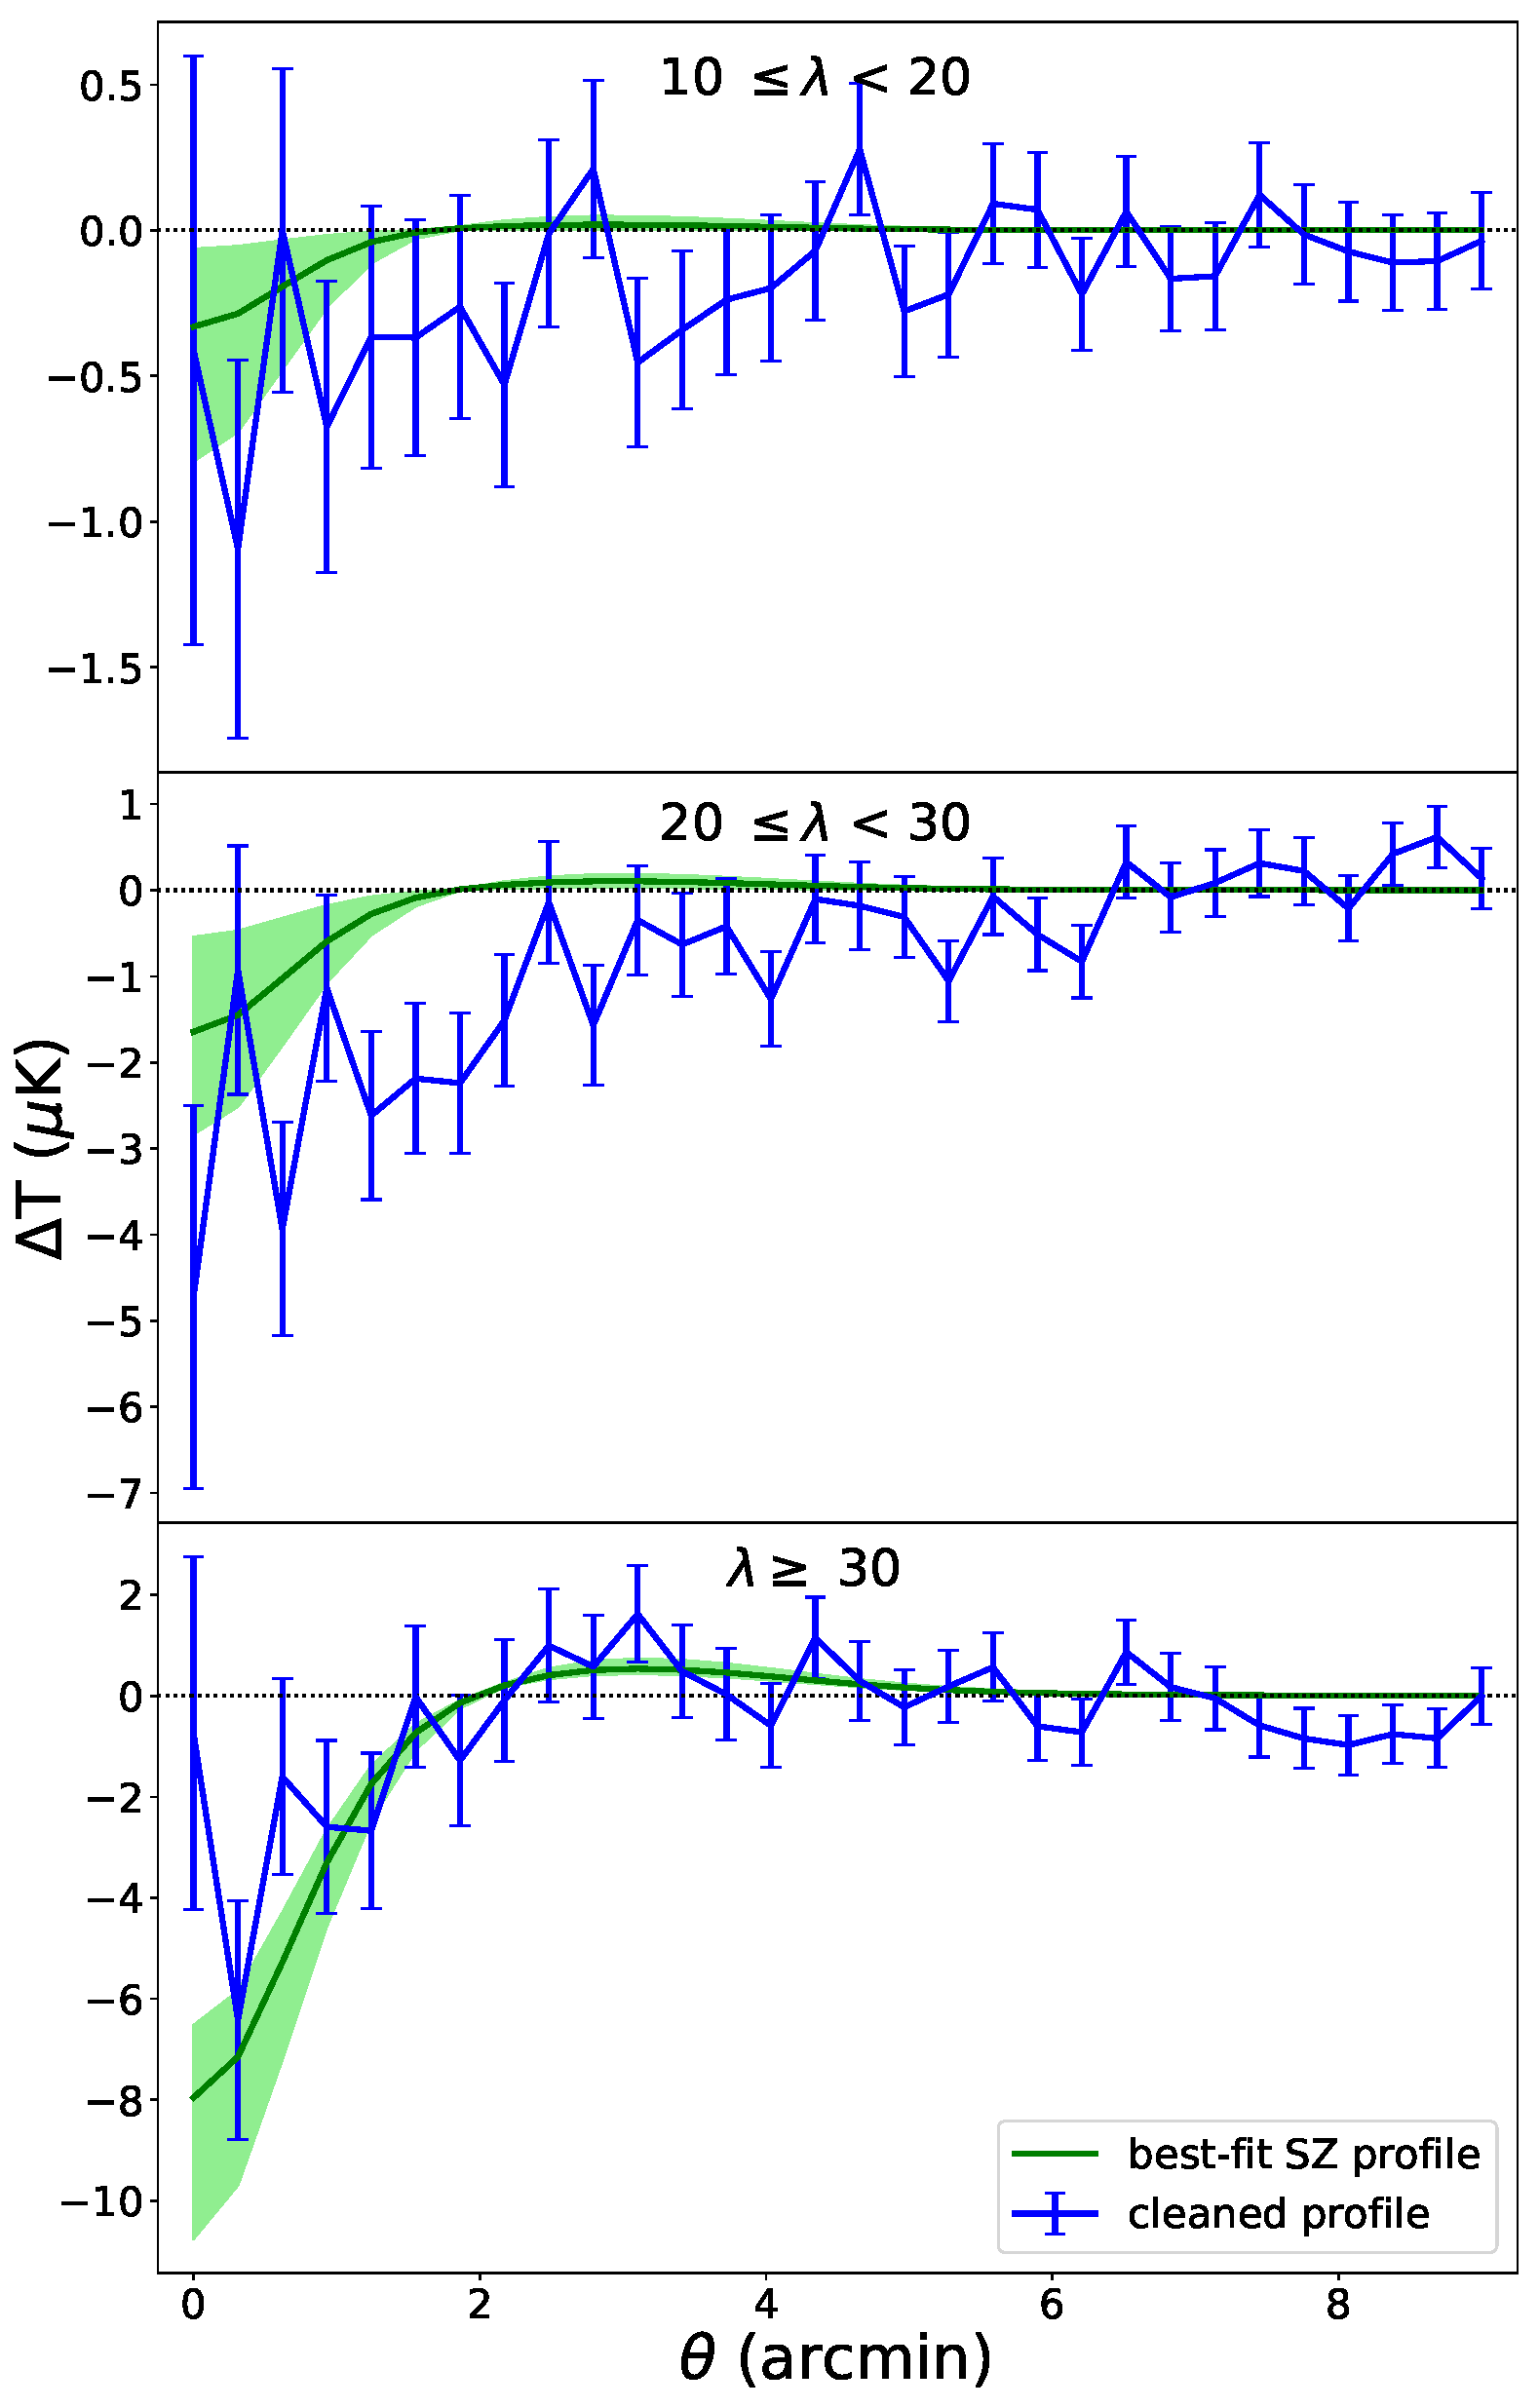
\includegraphics[width=0.5 \textwidth]{MLprof_ncut_all_20190123.pdf}
  \caption{Results at 148 GHz from fitting for a cleaned SZ profile for the three richness bins. The blue line is the stacked profile after subtracting the mean dust and radio emission profiles. The green line is the mean profile for the SZ model from the MCMC chains. The green contours bound the models in the chain between the 16th and 84th percentiles in each angular bin.}
  \label{fig:mcmcprof}
\end{figure}


%%%%%%%%%%%%%%%%param contours
\begin{figure}
  \centering
  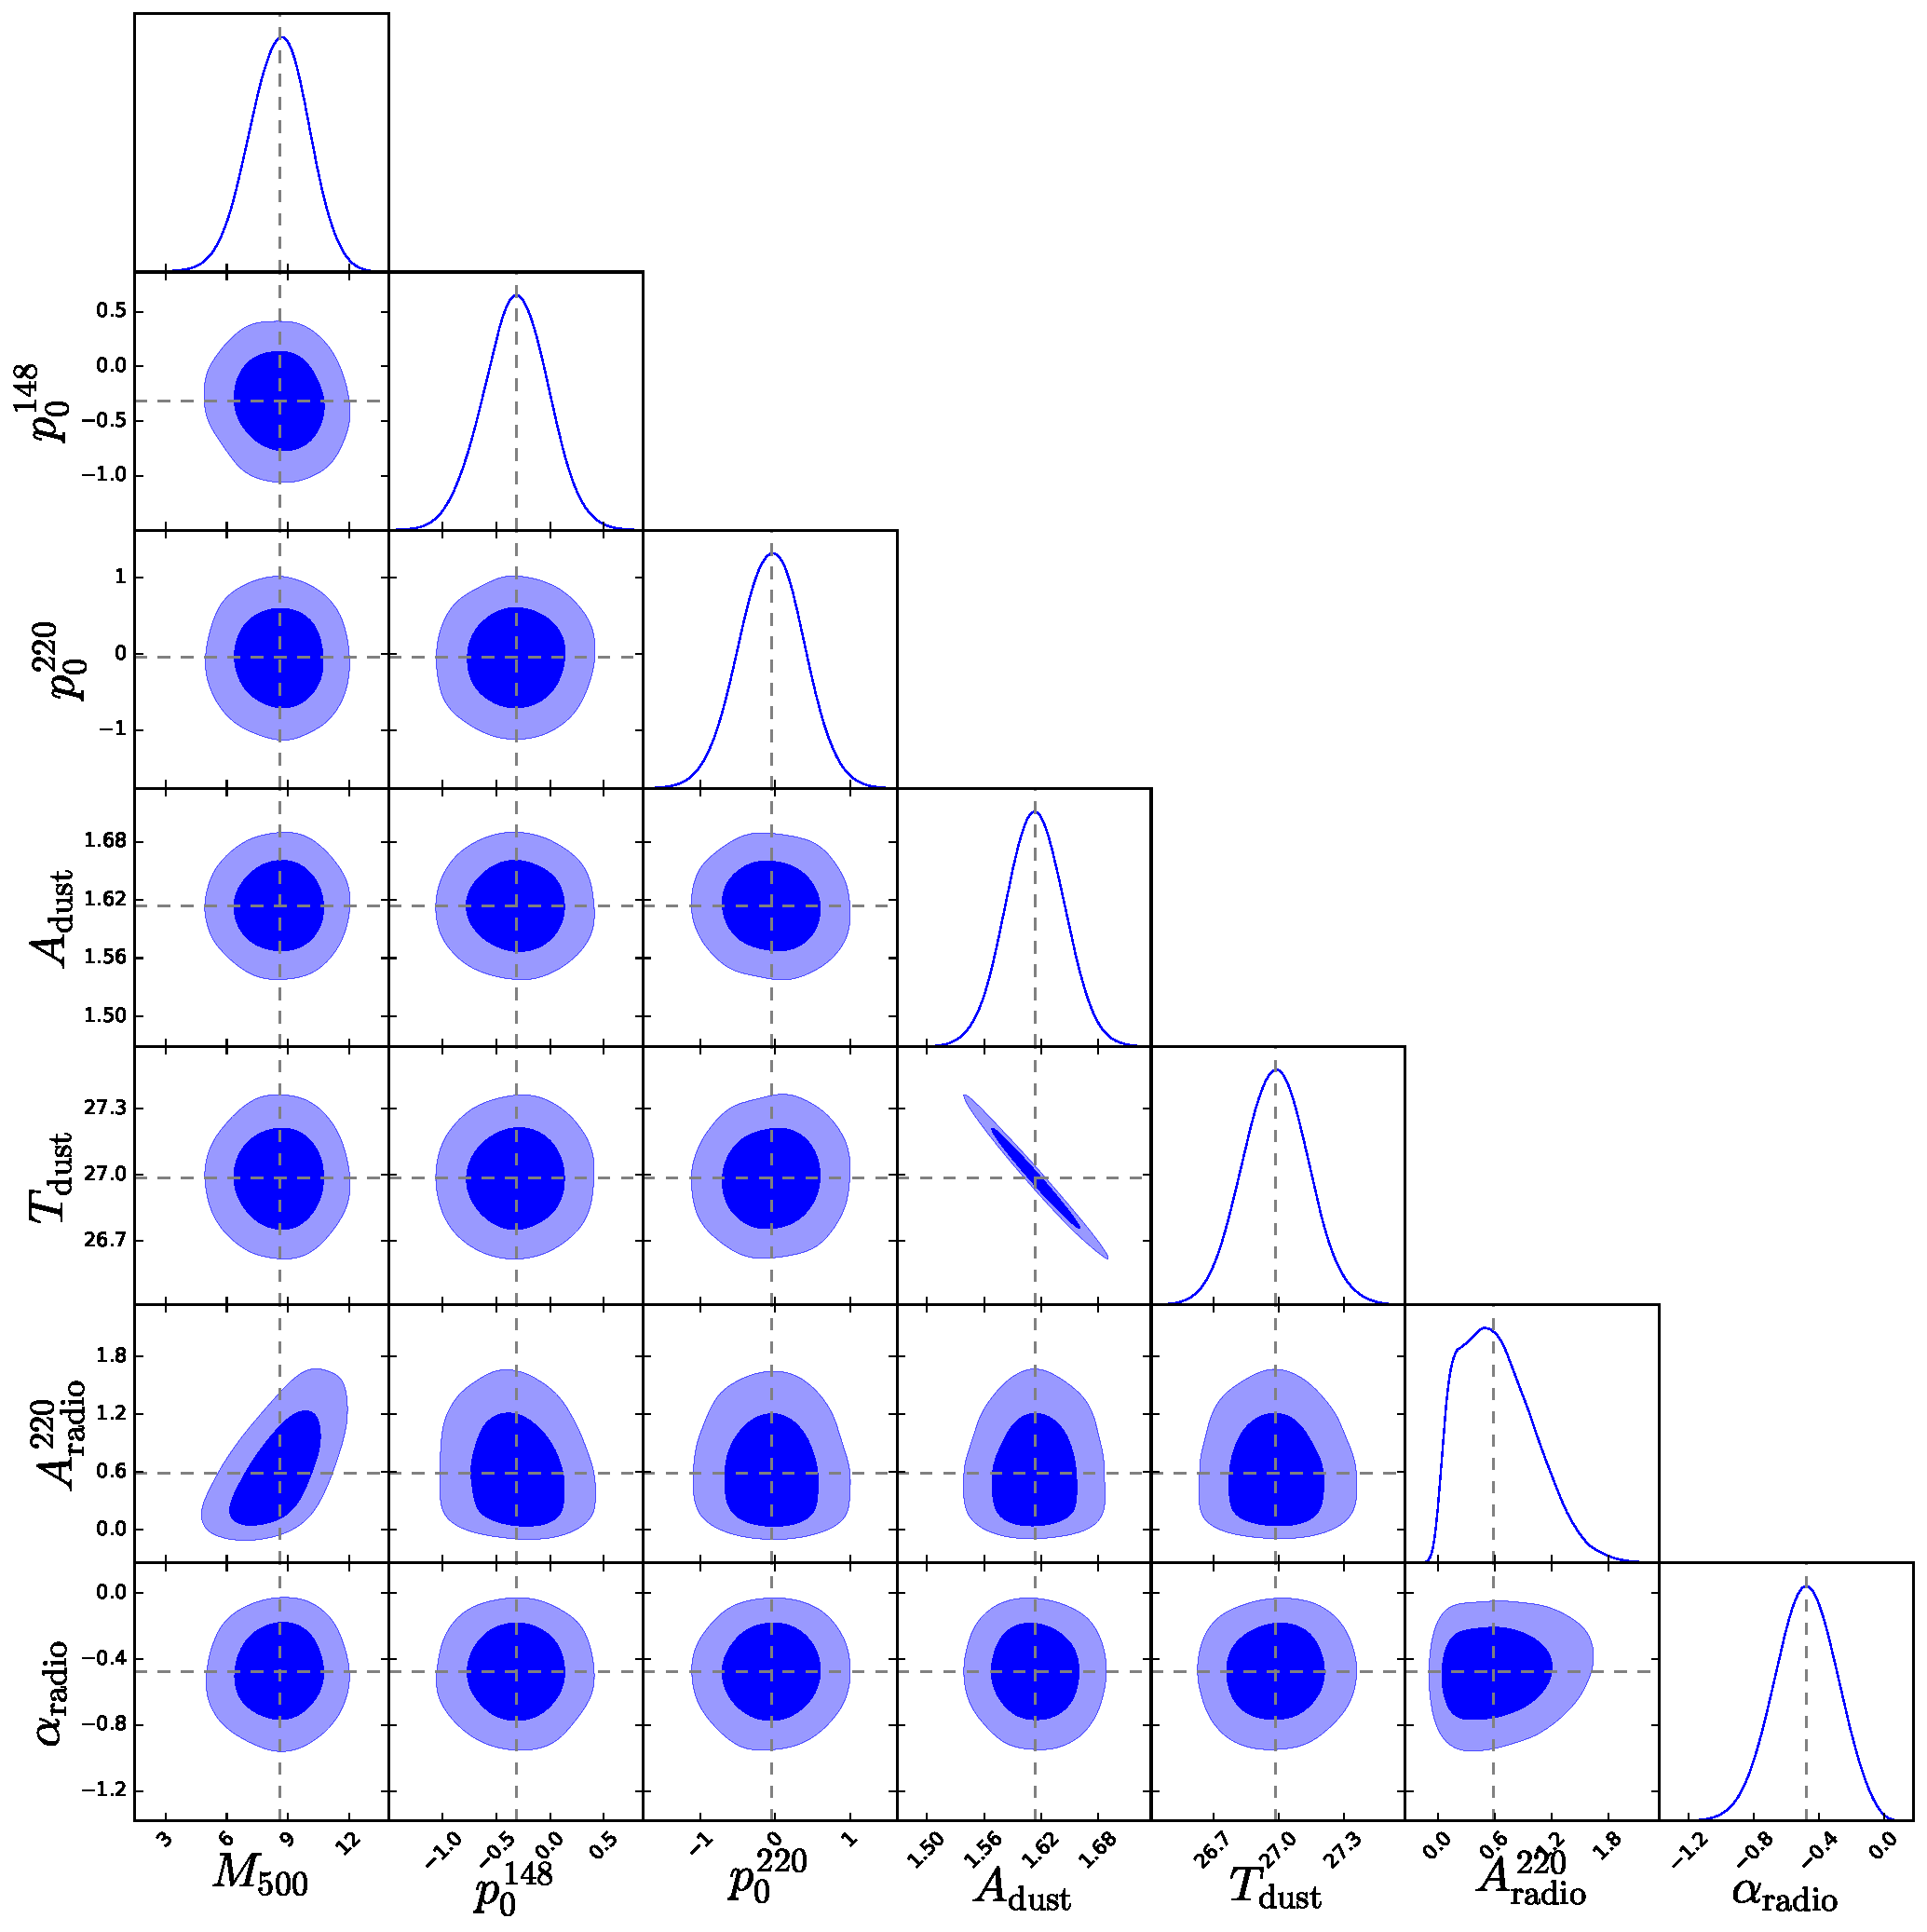
\includegraphics[width= \columnwidth] {corner_0190123_nw_18_ns_10000_mbatalpha_tophat_11_arcmin_zbin01_rbin2_v4_sigalpha02_numpy_cut_1000.pdf}
  \caption{Parameter contours from MCMC chains for the highest richness bin, $\lambda \geq 30$. The grey dashed lines pass through the mean value from the probability distributions for each parameter. The dust amplitude and temperature are anti-correlated in all richness bins.}  \label{fig:mcmccontours}
\end{figure}



Figures \ref{fig:mcmcprof} and \ref{fig:mcmccontours} show the results from fitting the stacked profiles for SZ, dust, and radio components. 
Figure \ref{fig:mcmcprof} shows one way to visualize the result, as the 148 GHz profiles, but cleaned of best-fit radio and dust emission models, along with the most likely SZ profiles from the MCMC chains. 
The light green area encompasses 68\% of the SZ models from the MCMC chains in each annular bin.  

The richest bin appears by eye to be a good fit, but the middle and lower richness bin show some residual decrement in the cleaned profile that is too broad to fit with an SZ profile.  
We have tested that increasing the mass worsens $\chi^2$ compared to the best fit model.  
Possible causes of this residual include large scale CMB fluctuations, or a possible oversubtraction of the dust or radio emission (which has also a somewhat extended profile compared to the SZ).  
If the dust and radio have been oversubtracted, then we will have over-estimated the masses of the halos in these bins.

For the highest richness bin, Figure \ref{fig:mcmccontours} shows the parameter contours for $M_{500}$, a DC offset in the 148 GHz stack, a dust spectrum amplitude, and a dust temperature, a radio spectrum amplitude, and the scaling for the radio spectrum from the MCMC chains. 
The radio amplitude, $A^{220}_{\rm radio}$, and the SZ mass are correlated. 
The parameter contours for the other richness bins are nearly identical.
The fit parameters are summarized in Table \ref{table:mcmcfitparam}, which show results from simultaneously fitting dust, radio, and SZ components to the ACT data, as well as fitting an SZ profile directly to the data while neglecting to correct for dust and radio emission. 
In the lowest richness bin, we do not make a significant mass measurement.
To better compare the relative magnitudes of the dust and radio signals, we report an amplitude at 220 GHz for the dust signal, which is computed by integrating the best-fitting dust profile at 220 GHz over the solid angle.
This makes it easier to see that the dust signal is more prominent than the radio.
The SZ mass is $M_{500} = 1.1^{+0.5}_{-1.1} \times 10^{13} \rm M_{\odot}$. 
The SZ mass measurement for the middle richness bin is $2.7^{+1.5}_{-1.4} \times 10^{13} \rm M_{\odot}$. 
In the highest richness bin, we measure an SZ mass of $8.6^{+1.6}_{-1.4} \times 10^{13} \rm M_{\odot}$. 
For the two higher richness bins, neglecting to correct for dust decreases the mass by 37\% for $20 \leq \lambda < 30$ and 23\% for $\lambda \geq 30$.

For a robustness check, we use the random stacks from Figure \ref{fig:randstacks} to test what mass our pipeline measures when there is no signal. 
Fitting without a dust correction results in probabilities of measuring a mass that pushes up against the lower limit of the prior (zero mass). 
At 95\% confidence, the upper limit of the null mass distributions are $2.0 \times 10^{13} \rm M_{\odot}$, $3.0 \times 10^{13} \rm M_{\odot}$, and $4.9 \times 10^{13} \rm M_{\odot}$, for the lowest to highest richness bins.
{The mean null stack masses are $1.2 \times 10^{13} \rm M_{\odot}$, $1.5 \times 10^{13} \rm M_{\odot}$, and $2.7 \times 10^{13} \rm M_{\odot}$, for the lowest to highest richness bins.}
%We also measure the SZ mass of only the dust correction (the case of zero SZ signal), using the data stack at 220 GHz as shown in Figure \ref{fig:rawstacks} and measure masses of $(1.7^{+0.9}_{-0.7}) \times 10^{13} \rm M_{\odot}$, $(2.1^{+1.2}_{-2.0}) \times 10^{13} \rm M_{\odot}$, and $(3.2^{+1.8}_{-1.9}) \times 10^{13} \rm M_{\odot}$ for the lowest to highest richness bins respectively. 
%For the highest richness bin, this demonstrates that correcting for dust contamination can have a significant effect on the measured masses of the clusters. For the lower richness bins, the measurements are not significant enough to draw a conclusion.



\subsection{Mass Bias}
The relation between SZ signal and cluster mass, $Y$--$M$, is often measured using X-ray derived cluster masses \citep{2010A&A...517A..92A, 2011ApJ...738...48A}, but there are several effects that cause these X-ray mass measurements to be biased low. 
Clusters are assumed to be in hydrostatic equilibrium (HE), but non-thermal pressure support from turbulence and random motions move the clusters away from perfect HE. 
The bias between the true mass and the mass measured by the SZ effect is quantified as $1-b = M_{\rm SZ}/M_{\rm true}$. The precise value for $1-b$ is not well understood and could lie in a large range \citep{2014A&A...571A..16P}. In \cite{2014A&A...571A..16P}, $1-b$ is fixed at 0.8. 
\cite{2016JCAP...08..013B} measured the mass bias for high-signal-to-noise clusters from the ACT equatorial survey, using weak-lensing data from the Canada-France-Hawaii telescope stripe 82 survey. 
They found that $1-b$ is 0.98 $\pm$ 0.28 and 0.87 $\pm$ 0.27 when fitting the weak-lensing mass using models based on simulations and an NFW profile, respectively. 
\cite{2018arXiv180405873M} present the amount of mass bias present in ACTPol clusters when comparing their SZ masses to weak lensing masses derived from Hyper-Suprime Cam data. They find $1-b = 0.74^{+0.13}_{-0.12}$.
There have been several other measurements of $1-b$, with values ranging from 0.58 to 0.95 \citep{2014MNRAS.443.1973V,2015MNRAS.449..685H,2016MNRAS.456L..74S,2016A&A...594A..24P}. 
When comparing our measured $M_{SZ}$ to cluster mass scaling relations, we use the values: $1-b = 1$, 0.8, and 0.6. 
We choose these values to sample the range of values that have been measured, so that we can demonstrate how much different amounts of mass bias could affect our mass measurements. 


\subsection{Richness to Mass Scaling}
\begin{figure}
  \centering
    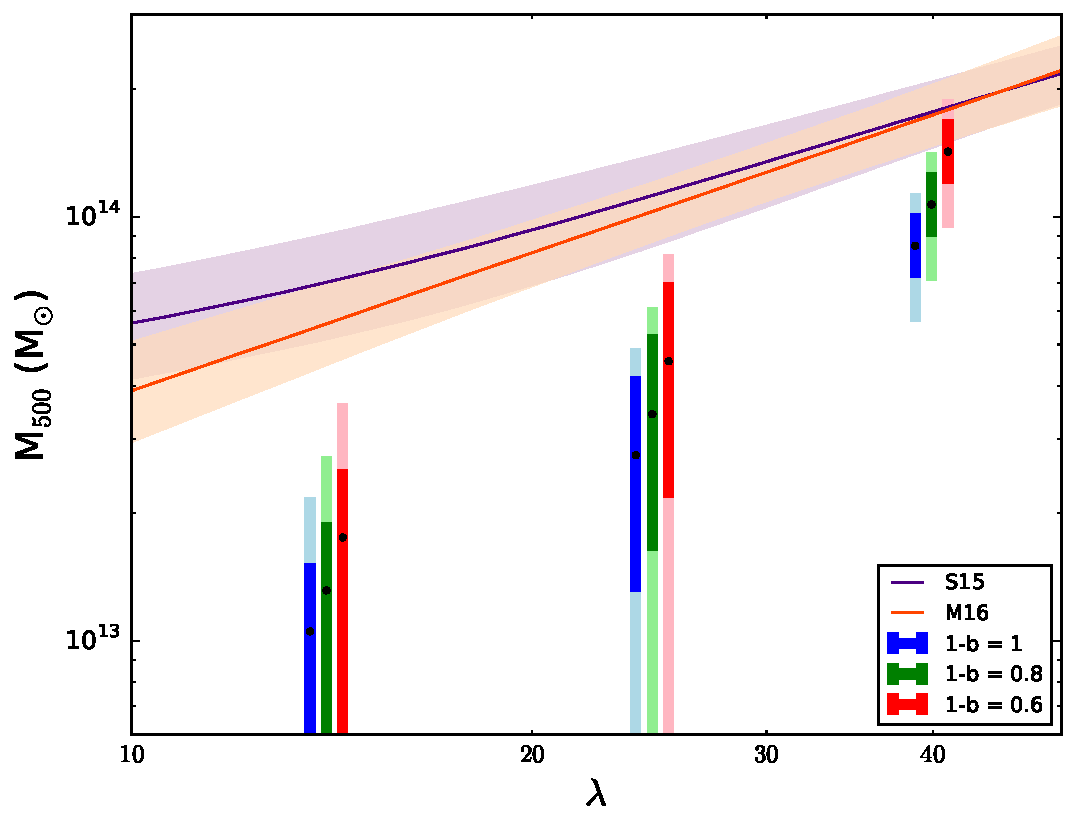
\includegraphics[width=\columnwidth] {M500_lambda_shela_sptvsrm_radiocorr.pdf}
  \caption{Comparison of SHELA SZ masses with redMaPPer mass-richness relations. The orange line is the mass-richness relation of \protect \cite{2016arXiv161006890M} which was calibrated using weak-lensing masses of redMaPPer clusters in DES data. The purple line is the mass-richness relation of \protect \cite{2015MNRAS.454.2305S} which was calibrated using SZ masses of redMaPPer clusters in SPT. For both models, the average redshift of all the clusters, z = 0.78, is used. The data points for the results for the masses of the SHELA clusters in each richness bin with different values for the amount of mass bias, $1-b$. The data point for the case of $1-b=1$ is plotted at the average richness in each bin. The other two points are slightly offset from the average richness for the sake of clarity. The error bars highlight 68\% and 95\% of the likelihood.}
  \label{fig:y500vslambda}
\end{figure}


We find that the SZ masses we measure are significantly smaller than those predicted by optical richness scaling relations. 
Accurately measuring the masses of cluster halos is necessary for clusters to be used for cosmology, making it vital to map out the relation between mass and the cluster observables, such as the SZ signal and richness. 
It is important to compare different observable to mass relations which have different biases and contaminating factors to test if predicted scaling relations hold. 
Multiple studies have seen that the SZ observable has some features that cause a lower SZ signal than predicted when $\lambda$--$M$ relations are extrapolated to lower mass objects \citep{2011A&A...536A..12P,2012PhRvD..85b3005D,2013ApJ...767...38S, 2017MNRAS.468.3347S}, and we explore that possibility here.  

For example, \cite{2017MNRAS.468.3347S} [S17] used a sample of DES redMaPPer clusters and measured their SZ signal by stacking in SPT (South Pole Telescope) data in multiple richness bins.  
They used their own richness-mass model from \cite{2015MNRAS.454.2305S} [S15], derived by cross-matching redMaPPer-detected clusters to SPT-detected clusters, and inverted it into a mass-richness model.
They ran two cases to relate the mass to the SZ signal, using their own $Y_{500} - M_{500}$ model and using the model from A10. 
They compared the $Y_{500}$ expected in each richness bin to what was measured from stacking on the SPT SZ map. They found that for clusters with $\lambda$ > 80, $Y_{500}$ is consistent with their model and smaller by 0.61$\pm$0.12 from A10. 
For 20<$\lambda$<80, they found that the SZ signal was smaller by a factor of ~0.2-0.8, with higher richness bins and the S15 $Y_{500} - M_{500}$ showing better agreement. 
They discuss possible explanations for this, such as a richness dependent bias caused by contamination of the SZ and richness observables. 
Another possibility they discuss is a bias in estimated halo mass. This could be caused by a contamination in the richness from line of sight projections, contamination of the SZ observable, a larger offset in SZ-optical centering than accounted for, or a larger intrinsic scatter in richness-mass relation at lower richness.

In Figure \ref{fig:y500vslambda} we compare our results to the $M_{500}$-$\lambda$ relation of S15. 
To make this comparison, we need to take into account that they have modeled $P(\lambda|M_{500})$ as opposed to $P(M_{500}|\lambda)$. 
Their model is a log-normal distribution with mean:
\begin{equation}
\langle \ln\lambda | M_{500},z\rangle = \ln A_{\lambda} + B_{\lambda} \ln\bigg(\frac{M_{500}}{3 \times 10^{14}h^{-1}\rm M_{\odot}}\bigg) + C_{\lambda}\ln\bigg(\frac{E(z)}{E(z=0.6)}\bigg)
\end{equation}
To invert this relation, we perform the following operation:
\begin{equation}
P(M_{500}|\lambda^{\rm obs}) \propto P(M_{500},z) \int P(\lambda^{\rm obs}|\lambda) \  P(\lambda|M_{500},z) \ d\lambda
\end{equation}
where $P(\lambda|M_{500},z)$ is the SPT probability marginalized over the fit parameters $A_{\lambda}$, $B_{\lambda}$, and $C_{\lambda}$. 
$P(\lambda^{\rm obs}|\lambda)$ is the probability for observing a value for the richness given the true richness, and $P(M_{500},z)$ is proportional to the halo mass function. 
This inverted relationship is used in Figure \ref{fig:y500vslambda} to compare against our SZ masses.


\cite{2016arXiv161006890M} [M16] measure $P(M_{200}|\lambda)$ for redMaPPer clusters in DES. 
For comparison, we translate their model in terms of $M_{200m}$ to $M_{500c}$, where $m$ denotes the density contrast relative to the mean matter density and $c$ is relative to the critical density at that redshift. 
This relation is plotted in Figure \ref{fig:y500vslambda}. 
Although we do not compare our data to other redMaPPer richness-mass models, we note that there is good agreement between relations from S15, \citet[][which is calibrated for clusters in SDSS]{2017MNRAS.466.3103S}, and \citet[][which is calibrated for clusters in DES Year 1 data]{2018arXiv180500039M}.

We compare the models from S15 as they used redMaPPer clusters with masses derived using the SZ effect, as are ours, and M16 as their redMaPPer richnesses are from data observed by DECam, similarly to the SHELA data. 
We do not expect the higher redshift range of our clusters to affect this comparison as there is no significant redshift evolution in either model. 
We plot our data against these models in Figure \ref{fig:y500vslambda}. For the SHELA sample, $M_{500}$ from SZ profile fitting and the average richness per bin are used. 
We tested different ways to represent our richness bins, such as using mass-weighted and SZ-weighted average richnesses, but find that they are similar to the mean richness per bin, so we simply use the mean value. 
The average richnesses for the bins are approximately 14, 24, and 39. 
Similarly to the results of S17, we find that the SZ decrements of our clusters indicate that they are less massive than predicted by their richnesses and the cluster mass-richness relationships.
Without accounting for mass bias for the highest richness bin, the predicted masses from S15 and M16 are 2.0 times larger than the SZ mass we found. 
With a  mass bias of $1-b = 0.6$, the predicted masses from S15 and M16 are 1.2 times larger. 
As is shown in Figure \ref{fig:y500vslambda}, a large value for mass bias would be necessary to reconcile our highest richness mass measurement with the richness-based mass models. 
The lower two richness bins have masses that are significantly below the predicted values, even when accounting for mass bias.
There would have to be a significant error in the richness to cause this large of a discrepancy, therefore there must be other factors in play. 
Most of the possible explanations coincide with those from the discussion in S17: more contamination in the SZ signal than we have accounted for, contamination in the richness estimate, and the mass-richness relations being incorrect at low richness. 
For the SHELA sample specifically, there could also be a differences in the meaning or interpretation of the richness, as the redMaPPer algorithm included IR data in addition to optical data when identifying this sample.

%%%%%%%%%%%%%%%%%%%%%%%%%%%%%%%%%

%%%%%%%%%%%%%%%%%%%%%%%%%%%%%%%
%CONCLUSIONS
%%%%%%%%%%%%%%%%%%%%%%%%%%%%%%%
\section{Discussion} \label{sec:conclusions}
We have presented the analysis of stacked SZ profiles for a sample of IR and optically-selected clusters from the Spitzer-HETDEX Exploratory Large Area survey. 
We split this sample into three richness bins: $10 \leq \lambda < 20$, $20 \leq \lambda < 30$ and $\lambda \geq 30$. There are 840, 172, and 70 clusters in the richness bins, from lowest to highest. 
At the SZ null (220 GHz), the stacked profiles exhibited an excess signal, which we attributed to dust and radio emission from cluster member galaxies. 
For each bin, we fit for a dust SED using sources from the Herschel Stripe 82 survey catalog to extrapolate the Herschel stacks to 148 and 220 GHZ. 
We also fit for a radio amplitude while setting a prior on the radio spectral index, which we use to find the contributions from radio emission at 148 and 220 GHz. 
We fit for an SZ profile using a universal galaxy cluster pressure profile to translate our temperature decrement to a halo mass. 
For each richness bin, we used an MCMC procedure that simultaneously fit for the SZ, dust, and radio components while fixing the redshift to the average of the cluster sample.  
We compared the chains with and without the dust and radio correction, and found on average that correcting for dust emission increases the $M_{500}$ measurement by a factor of 1.4. 


The SHELA cluster catalog obtains richnesses from the redMaPPer algorithm. 
We compared our SZ mass and richness data to two models which have mapped out the richness-mass relation for redMaPPer clusters. 
SZ measurements of optically-selected clusters are generally smaller than expected when comparing to mass-richness models, and the SHELA clusters follow this trend. 
For all three richness bins, it would take a large amount of mass bias to reconcile our measurements with redMaPPer mass-richness relations. 
For the $\lambda \geq 30$ bin, the masses predicted by mass-richness relations are 2.0 times larger than our SZ mass.
Taking into account a mass bias value of $1-b = 0.6$, the predicted masses are 1.2 times larger.
For the lower two richness bins, our SZ mass measurements fall below the predicted masses even when taking mass bias into account.

This work is a step toward studying characteristics of galaxy clusters over a range of redshifts and masses. 
In the future, wider and deeper coverage by Advanced ACT and the Simons Observatory will advance this study by observing a large number of clusters in five frequency bands, and by increasing overlap with optical surveys such as BOSS, HSC, DES, DESI, and LSST \citep{2016SPIE.9910E..14D}. 
It may be fruitful to repeat this type of analysis for more infrared-selected objects. A similar study could be done using the Spitzer IRAC Equatorial Survey \citep[SpIES,][]{2016ApJS..225....1T} which is shallower than SHELA, but larger, covering an adjacent $\sim$115 square degrees of Stripe 82, or using the MaDCoWS cluster catalog which covers the full extragalactic sky at 0.7 $\lesssim z \lesssim 1.5$ \citep{2018arXiv180906820G}.

\section*{Acknowledgments}
BJF and KMH acknowledge support by the National Aeronautics \& Space Administration through the University of Central Florida's NASA Florida Space Grant Consortium and Space Florida. LK and CP acknowledge support from the National Science Foundation through grants AST 1413317 and 1614668. This work was supported by the U.S. National Science Foundation through awards AST-0408698 and AST-0965625 for the ACT project, as well as awards PHY-0855887 and PHY-1214379. Funding was also provided by Princeton University, the University of Pennsylvania, and a Canada Foundation for Innovation (CFI) award to UBC. ACT operates in the Parque Astron\'omico Atacama in northern Chile under the auspices of the Comisi\'on Nacional de Investigaci\'on Cient\'ifica y Tecnol\'ogica de Chile (CONICYT). Computations were performed on the GPC supercomputer at the SciNet HPC Consortium. SciNet is funded by the CFI under the auspices of Compute Canada, the Government of Ontario, the Ontario Research Fund - Research Excellence; and the University of Toronto. The development of multichroic detectors and lenses was supported by NASA grants NNX13AE56G and NNX14AB58G. We thank our many colleagues from ABS, ALMA, APEX, and Polarbear who have helped us at critical junctures. Colleagues at AstroNorte and RadioSky provide logistical support and keep operations in Chile running smoothly. We also thank the Mishrahi Fund and the Wilkinson Fund for their generous support of the project. %MCMC parameter contours were plotted using the python package \textit{corner} \citep{corner}.
LK and CP acknowledge support from the National Science Foundation through grants AST 1413317 and 1614668.

%%%%%%%%%%%%%%%%%%%%%%%%%%%%%%%%%%%%%%%%%%%%%%%%%%

%%%%%%%%%%%%%%%%%%%% REFERENCES %%%%%%%%%%%%%%%%%%

% The best way to enter references is to use BibTeX:

\bibliographystyle{mnras}
\bibliography{shela_sz} 


%%%%%%%%%%%%%%%%%%%%%%%%%%%%%%%%%%%%%%%%%%%%%%%%%%


% Don't change these lines
\bsp	% typesetting comment
\label{lastpage}
\end{document}
